\chapter{User Documentation}

In this chapter we will explore the usage of the program from the perspective of and end user. We define the minimum requirements for the programs running, provide ways for installation and show example usages of the program.

\section{Program requirements}

The program can run on any 64 bit processor and is prepared to run on Windows and Linux operating system. The program can run with only a \ac{CPU} but for it to work with OpenGl it needs a \ac{GPU} that is capable to run atleast 1024 concurrent threads. The CUDA functionality requires an NVIDIA \ac{GPU} whit the same concurrent thread requirement.

\section{Installation guide}

The program requires no installation for an end user. You only need to download the provided compressed binaries for your operating system from the following website \hyperref{https://github.com/Palnit/BSC-Thesis}{https://github.com/Palnit/BSC-Thesis} and unzip the binary and run. Currently there's 4 compiled binary: linux, linux-no-cuda, windows, windows-no-cuda. The no-cuda version binaries were created so the program can run on non CUDA compatible GPUs. If you want to build it for your self with CUDA capability you need to download the CUDA SDK from \hyperref{test}{test} and CMAKE with a \CC\ build system e.g.: ninja, make and a compiler e.g.: \GG\ , MSVC, Clangd. There's two standalone programs one is for synthetic testing the other is for testing on real pictures. The synthetic tester's name is: BSC\_Thesis\_Tests, the real picture tester's name is: BSC\_Theis. 

\begin{figure}[H]
\begin{minipage}{.49\textwidth}
\begin{figure}[H]
\centering
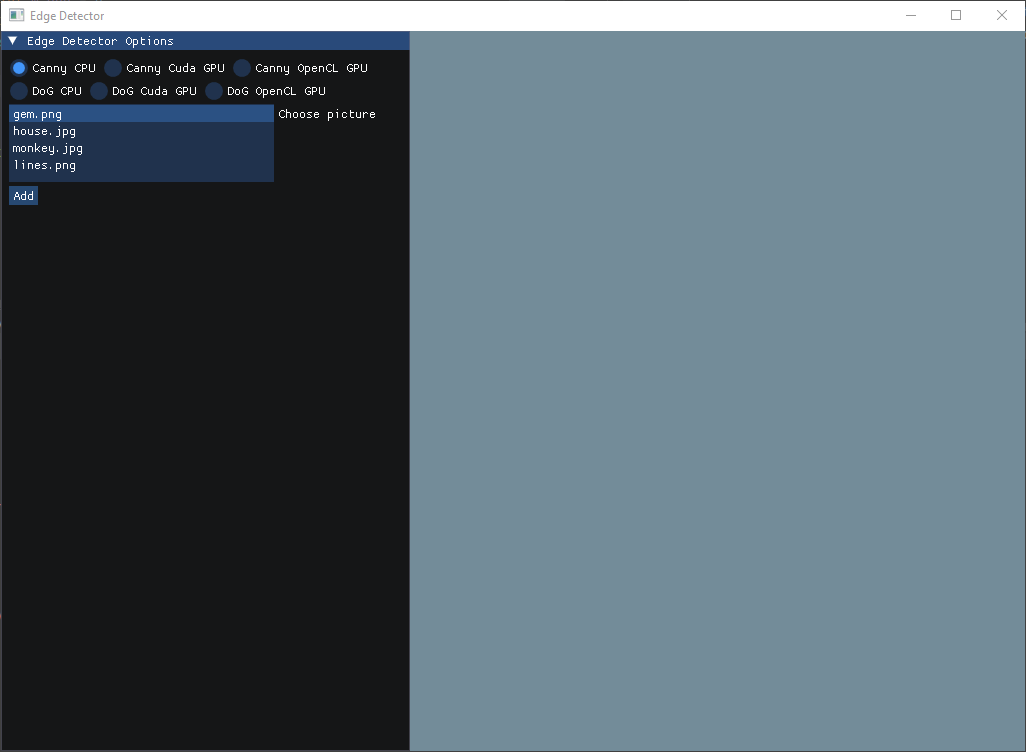
\includegraphics[width=\linewidth]{picture_window}
\caption{Program for real pictures}
\label{fig:noraml_prog}
\end{figure}
\end{minipage}
\begin{minipage}{.49\textwidth}
\begin{figure}[H]
\centering
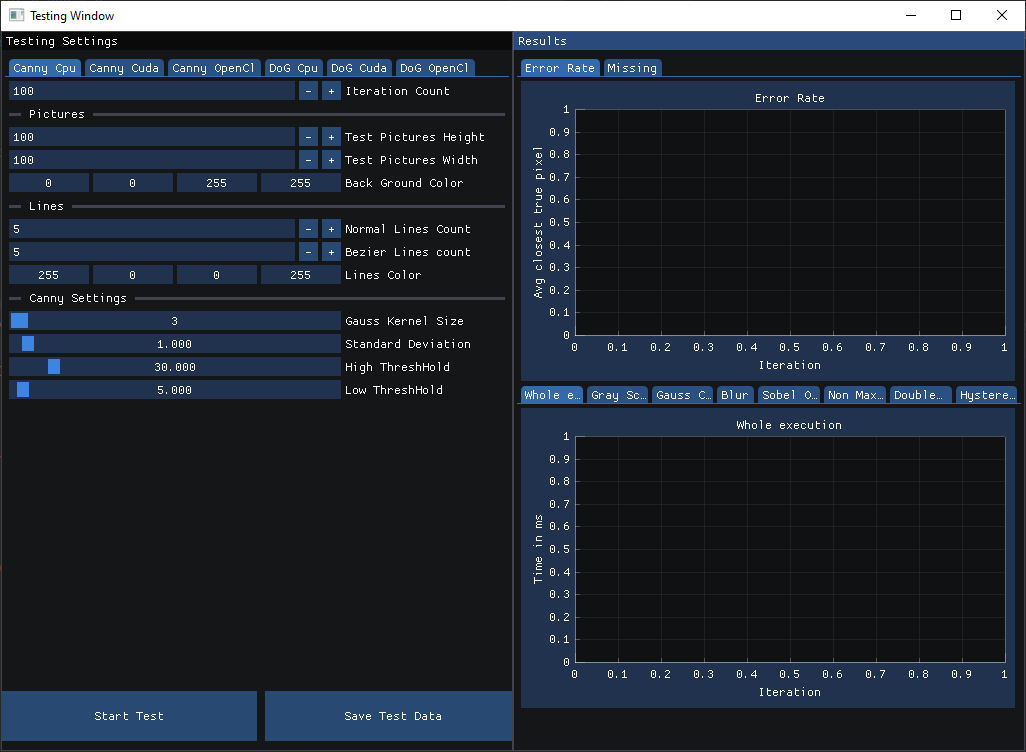
\includegraphics[width=\linewidth]{sintetic_tester}
\caption{Program for synthetic testing}
\label{fig:test_prog}
\end{figure}
\end{minipage}
\end{figure}

\section{Program Introduction}

In this section I will now demonstrate how the two programs work how to use them and what can what errors might occur during the usage of our program.

\subsection{Synthetic Tester}
\label{chap:tester}

\begin{figure}[H]
\centering
\begin{minipage}[t]{.49\textwidth}
\centering
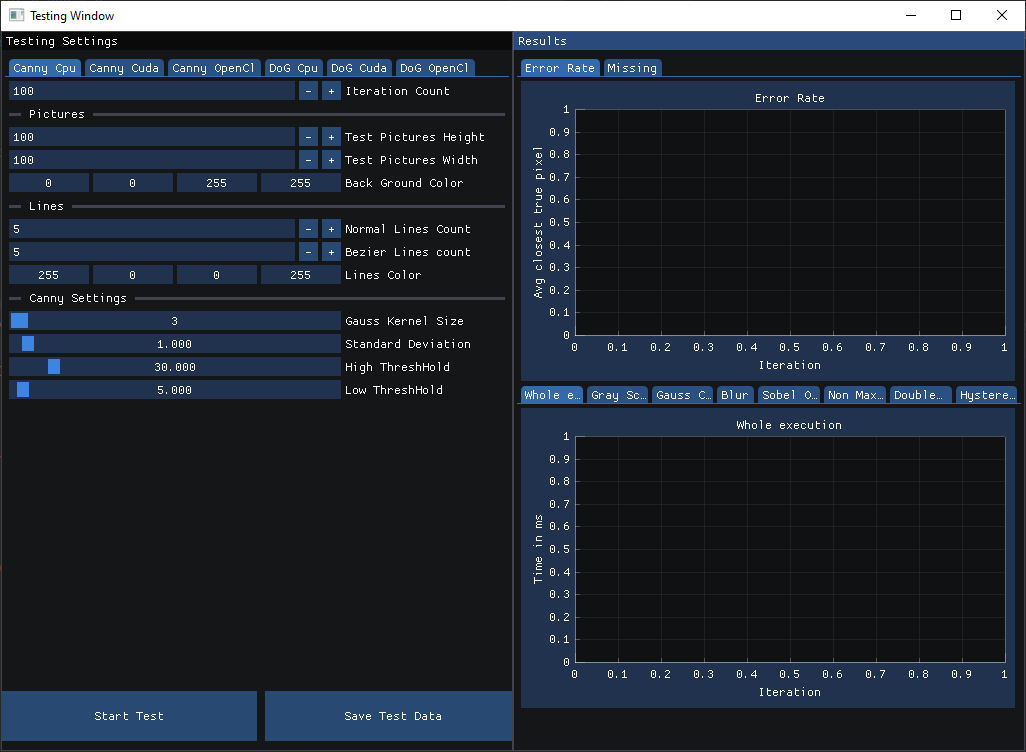
\includegraphics[width=\linewidth]{sintetic_tester}
\end{minipage}
\begin{minipage}[t]{.49\textwidth}
\centering
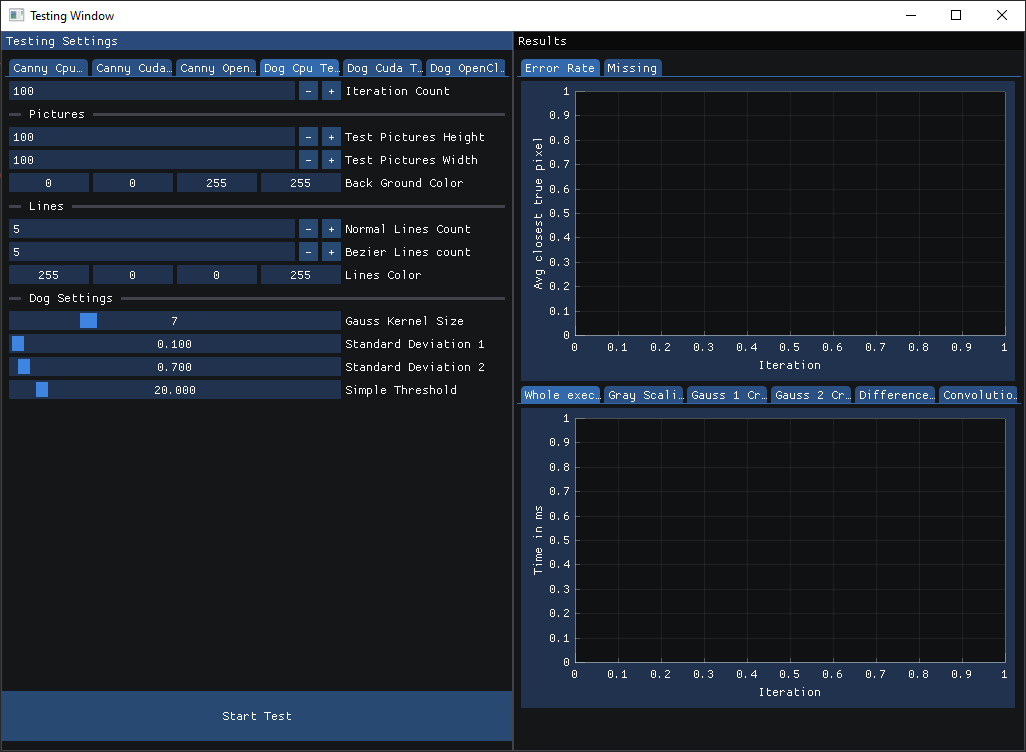
\includegraphics[width=\linewidth]{sintetic_tester_dog}
\end{minipage}
\caption{Difference between the settings of \ac{Canny} and \ac{DoG} detection pages}
\label{fig:test_prog_dem}
\end{figure}

For the synthetic tester we can see in \autoref{fig:test_prog_dem} in both pictures at the left side of the window are the settings for the tester. At the top we can choose which detector we want to test. Below that we can choose the test pictures settings we can set it's height, width, and base color. After that we can see the settings for the lines how many normal and curved lines we want and what color should they be. And lastly we can see the specific settings for the algorithm. 

If we choose to test the \ac{Canny} algorithm as we can see on the left picture in Figure \ref{fig:test_prog_dem} there are 4 settings. The kernel size of the Gaussian blur, the standard deviation of sad kernel, and the high/low thresh holds of the \ac{Canny} algorithms this adjusts what pixel values should be kept these are kept low for the purpose to find the most pixels for the tests. 

As for the \ac{DoG} algorithm if we take a look at the right picture in \autoref{fig:test_prog_dem} there's 4 settings too. The first is the same kernel size as in \ac{Canny} algorithm this will set the size for bot kernels used in the algorithm. Below that there's to standard deviation for the two kernel's that will be used. And lastly there's a Simple threshold to be able to test accuracy, this is original not a part of the algorithm but we need it to be able to differentiate between detected pictures and undetected pictures because their values are not exact

This settings are needed to adjusts the algorithms to get the best results. Sadly we cannot write an algorithm that will find the edges that our human minds register and there can be many errors these settings are there to help make pictures clearer.

And lastly there's a button on the bottom of the page that will start the testing.

For the right side of the window where we will see the test results data. at the top we can see the error rate and the missing pixel count. The error rate show for each iteration of the program how many pixels were detected that are not actual pixels. The missing pixels show how many of the original pixels from the lines were not detected in at all. Below these two we can see the graph for the timings. Here we can take a look at how many \ac{ns} it took the program to finish each step of the algorithm.

\subsection{Real picture tester}




